
\documentclass[11pt]{bredelebeamer}
  \usepackage{booktabs} 
  \usepackage{multirow}
\usepackage{array}
\usepackage[]{color}
\usepackage{blkarray}
\usepackage{tikz}
\usepackage{verbatim}
\usepackage{amsmath,graphicx,centernot}
\usepackage{lipsum}
\usetikzlibrary{arrows,shapes}
\usetikzlibrary{arrows.meta}
\usepackage{subcaption}
\captionsetup{compatibility=false}
\usetikzlibrary{shapes,backgrounds,arrows,automata,snakes,shadows,positioning, mindmap}
\usepackage{amsmath,amssymb,amsthm,mathrsfs,amsfonts,dsfont} 
\usepackage{color, colortbl}
\newcommand\independent{\protect\mathpalette{\protect\independenT}{\perp}}
\renewcommand{\newblock}{}
\def\independenT#1#2{\mathrel{\rlap{$#1#2$}\mkern2mu{#1#2}}}
\tikzset{
  level/.style   = { ultra thick, blue },
  connect/.style = { dashed, red },
  notice/.style  = { draw, rectangle callout, callout relative pointer={#1} },
  label/.style   = { text width=2cm }
  rect/.style = {rectangle, rounded corners, draw=black,
                           minimum width=4cm, minimum height=1cm,
                           text centered, font=\sffamily}
  connect/.style = { dashed, blue }
}


\newcommand{\backupbegin}{
   \newcounter{framenumberappendix}
   \setcounter{framenumberappendix}{\value{framenumber}}
}
\newcommand{\backupend}{
   \addtocounter{framenumberappendix}{-\value{framenumber}}
   \addtocounter{framenumber}{\value{framenumberappendix}} 
}
\DeclareMathOperator*{\argmax}{arg\,max}
%%%%%%%%%%%%%%%%%%%%%%%%%%%%%%%%%%%%%%%%%%%%%%%%



\title[Inférence de réseaux]{Inférence de réseaux écologiques à partir d'arbres latents dans un modèle Poisson Log-Normal}
\subtitle{Encadré par  S. Robin$^{\inst{1}}$ et C. Ambroise$^{\inst{1}\inst{2}$ }}

\institute[]
{
  \inst{1}%
  UMR AgroParisTech / INRA MIA-Paris \\
  \inst{2}%
  LaMME, Evry
  }



\author{Raphaëlle Momal}
% La commande \inst{...} Permet d'afficher l' affiliation de l'intervenant.
% Si il y a plusieurs intervenants: Marcel Dupont\inst{1}, Roger Durand\inst{2}
% Il suffit alors d'ajouter un autre institut sur le modèle ci-dessous.




\date{\today}
% Optionnel. La date, généralement celle du jour de la conférence

\subject{Inférence de réseaux}
% C'est utilisé dans les métadonnes du PDF




%%%%%%%%%%%%%%%%%%%%%%%%%%%%%%%%%%%%%%%%%%%%%%%%%%%%%%%%%%%%%%%%%%%%%

\begin{document}
\begin{frame}
  \titlepage
\end{frame}
\section{Introduction}


\begin{frame}{Exemple de réseau écologique}
\begin{columns}
\begin{column}{0.45\linewidth}

\cite{jakuch}:\\


\begin{itemize}
\item But : à partir de mesures d'abondance, identifier les liens de dépendance entre le champignon \textit{E. alphitoïde} présent sur les feuilles du chêne, et les autres micro-organismes présents.\vspace{0.4cm}
\item Utile à la compréhension et au contrôle des maladies chez le chêne.
\end{itemize}

\vspace{0.4cm}
%Variable continue, structure de dépendance modélisée par des copules %gaussiennes utilisant les résidus de Pearson, puis inférence bayésienne du %réseau.
\end{column}
\begin{column}{0.55\linewidth}
\begin{figure}
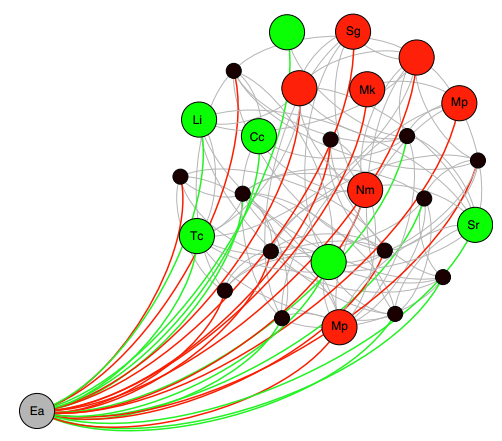
\includegraphics[scale=0.45]{illu_reseau.png}
\caption{Model of the pathobiome \textit{Erysiphe alphitoides} on oak leaves, source : Jakuschkin \textit{et al.} }
\end{figure}
\end{column}
\end{columns}

\end{frame}

\begin{frame}{Notion de réseau}
    \begin{itemize}
    \item Tableau de données observées Y de dimensions $n\times d$
    \begin{itemize}
        \item abondances de $d$ espèces, expressions RNA-seq de $d$ gènes ...\vspace{0.3cm}
    \end{itemize}
    
     \item Réseau : représentation graphique de la structure de dépendance conditionnelle du jeu de données.\vspace{0.3cm}
     
      \item Inférer un réseau : inférer les arêtes du graphe, \textit{i.e.} la structure de dépendance des variables (espèces, covariables, ...) de Y
    \end{itemize}

    \vspace{0.5cm}
\begin{columns}
 \begin{column}{0.35\linewidth}
 
Exemple : $Y=(Y_1,...,Y_4)$ : \\
 \begin{flushright}
 \begin{tikzpicture}
     

      %% UN graphe 
      \tikzstyle{every edge}=[-,>=stealth',shorten >=1pt,auto,thin,draw]
      \tikzstyle{every node}=[fill=yellow!40!orange]
      \tikzstyle{every state}=[draw=none,text=black,scale=0.5,
      transform shape,circular drop shadow] 
      
      \node[fill=white] at (2.25,-0.5) ;

      % premier cluster
      \node[state] (A1) at (1.,0) {$Y_1$};
      \node[state] (A2) at (2.8,0.7) {$Y_2$};
      \node[state] (A3) at (1.7,1.5) {$Y_3$};
      \node[state] (A4) at (2,0.7) {$Y_4$};
      
        \path (A2) edge [] (A4)
        (A1) edge [] (A4)
        (A3) edge [] (A4)
        (A3) edge [] (A1);
      

\end{tikzpicture}\\
\end{flushright}
\end{column}
\begin{column}{0.1\linewidth}
\begin{center}
\vspace{-0.5cm}
 $\Rightarrow$
\end{center}
\end{column}

\begin{column}{0.55\linewidth}
\begin{flushleft}
 \vspace{-0.5cm}
 Les variables $Y_2$ et $Y_1$ sont indépendantes entre elles conditionnellement à la variable $Y_4$.
\end{flushleft}

\end{column}

\end{columns}


\end{frame}



%\begin{frame}{Sommaire}
%  \tableofcontents
%  % possibilité d'ajouter l'option [pausesections]
%\end{frame}





\begin{frame}{Cadre mathématique: modèles graphiques }
\begin{itemize}
\item Clique $C$ d'un graphe $G$: sous-ensemble de noeuds de $G$ qui sont tous liés entre eux.\\

\item Clique maximale $C_{G}$ : aucune autre clique de $G$ ne la contient strictement.\\

\end{itemize}

\begin{exampleblock}{Propriété de factorisation \cite{Lau96}}
Soit  $Y = (Y_1,...,Y_q)$ et $p$ sa densité. $p$ se factorise selon le graphe non orienté G si :
\[ p(y) \propto \prod_{C \in C_G} \Phi_C (y^C) \]
Et alors G représente la structure d'indépendance conditionnelle entre les $Y_i$.
\end{exampleblock} 
\begin{columns}
 \begin{column}{0.35\linewidth}
 \begin{flushright}
\vspace{0.3cm}
 \begin{tikzpicture}
     

     \tikzstyle{every edge}=[-,>=stealth',shorten >=1pt,auto,thin,draw]
      \tikzstyle{every node}=[fill=yellow!40!orange]
      \tikzstyle{every state}=[draw=none,text=black,scale=0.5,
      transform shape,circular drop shadow] 
      
      \node[fill=white] at (2.25,-0.5) ;

      % premier cluster
      \node[state] (A1) at (1.,0) {$Y_1$};
      \node[state] (A2) at (2.8,0.7) {$Y_2$};
      \node[state] (A3) at (1.7,1.5) {$Y_3$};
      \node[state] (A4) at (2,0.7) {$Y_4$};
      
        \path (A2) edge [] (A4)
        (A1) edge [] (A4)
        (A3) edge [] (A4)
        (A3) edge [] (A1);
\end{tikzpicture}\\
\end{flushright}
 \end{column}
 \begin{column}{0.6\linewidth}
 \begin{flushleft}
    $p(Y) = \phi_1(Y_2,Y_4) \times \phi_2(Y_1,Y_3,Y_4)$
 \end{flushleft}
 \end{column}
\end{columns}
\end{frame}

\begin{frame}{\textit{Gaussian Graphical Models} (GGM)}
$Y$ une variable gaussienne multivariée de dimension $d$:
\vspace{0.3cm}
\begin{center}
  $Y=(Y_1,...,Y_d) \sim \mathcal{N}_d(0,\Omega^{-1})$,\\
$\Omega  = (\omega_{ij})_{ i,j }$. \\
\end{center}
 \vspace{0.3cm}
 L'écriture de la gaussienne permet directement d'obtenir une factorisation :

\begin{align*}
p(y) &\propto exp(-y^T \Omega y /2)\\
&\propto \prod_{j,k, \omega_{jk} \neq 0 } exp(-y_j \omega_{jk} y_k /2)  
\end{align*}
\pause{ \vspace{-1cm}
 \begin{columns} 
 \begin{column}{0.5\linewidth}

 \begin{flushright}
\[\Omega=
\left(
\begin{array}{*{4}{c}}
* & 0 & * & *\\
0 & * & 0 & *\\
* & 0 & * & *\\
* & * & * & *
\end{array}
\right)
\]
 \end{flushright}
 \end{column}
 \begin{column}{0.05\linewidth}
\begin{center}
 $\Rightarrow$
\end{center}
\end{column}
 \begin{column}{0.45\linewidth}
 \begin{flushleft}
\vspace{0.8cm}
 \begin{tikzpicture}
     

      \tikzstyle{every edge}=[-,>=stealth',shorten >=1pt,auto,thin,draw]
      \tikzstyle{every node}=[fill=yellow!40!orange]
      \tikzstyle{every state}=[draw=none,text=black,scale=0.5,
      transform shape,circular drop shadow] 
      
      \node[fill=white] at (2.25,-0.5) ;

      % premier cluster
      \node[state] (A1) at (1.,0) {$Y_1$};
      \node[state] (A2) at (2.8,0.7) {$Y_2$};
      \node[state] (A3) at (1.7,1.5) {$Y_3$};
      \node[state] (A4) at (2,0.7) {$Y_4$};
      
        \path (A2) edge [] (A4)
        (A1) edge [] (A4)
        (A3) edge [] (A4)
        (A3) edge [] (A1);
      

\end{tikzpicture}\\
\end{flushleft}
 \end{column}

\end{columns}}
\end{frame}

\begin{frame}{Inférence de $\Omega$ : le graphical Lasso}
\begin{itemize}

 \item La log-vraisemblance de  $Y$ s'écrit :
 \[L(Y,\Omega) = \frac{n}{2}\log(det(\Omega))-\frac{n}{2} Y^T\Omega Y + cste\]

 \item  Estimation parcimonieuse
\end{itemize}
 \begin{exampleblock}{ Le graphical-Lasso (glasso) :}
  Le graphical-Lasso pénalise la norme $l_1$ de la matrice de précision :
  \[\widehat{\Omega}_\lambda = \arg\min_{\Omega \in \mathcal{S}_d^+}\left\{ L(Y,\Omega)+\lambda \sum_{i\neq j} |w_{ij}| \right\}\]
 \end{exampleblock}
 \begin{itemize}
  \item Choix du $\lambda$...
 \end{itemize}

\end{frame}
\section{Modèle}

\begin{frame}{Données structurées par arbre}
\begin{columns}
 \begin{column}{0.7\linewidth}
 \begin{itemize}
    \item La structure de dépendance des données s'appuie sur un arbre \vspace{1cm}
    \item La vraisemblance des données se factorise sur les noeuds et les arêtes \cite{ChowLiu}:
    \end{itemize}
 \end{column}
 \begin{column}{0.3\linewidth}
 \begin{center}
     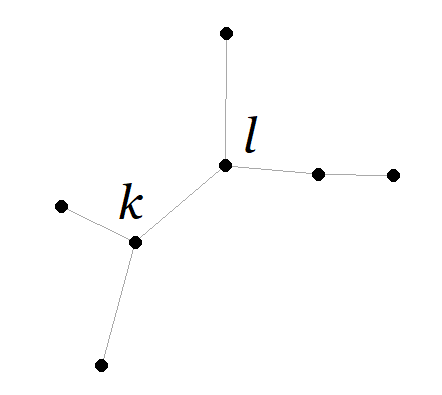
\includegraphics[width=3cm]{arbredependance.PNG}   
    \end{center}
 \end{column}
\end{columns}

\[\mathds{P}(Y|T) =\prod_{j=1}^d \mathds{P}(Y_j)\prod_{k,l \in T}\psi_{kl}(Y) \hspace{0.3cm},\]

Où \[ \psi_{kl}(Y) = \frac{\mathds{P}(Y_k,Y_l)}{\mathds{P}(Y_k)\times \mathds{P}(Y_l)}.\]\\
\vspace{0.4cm}
\textbf{Rmq} : dans le cas gaussien, $\hat{\Psi} = [\hat{\psi_{kl}}] = (1-\hat{\rho}^2)^{-1/2}$
\end{frame}
\begin{frame}{Loi Poisson Log-Normale (PLN)}
    
\begin{exampleblock}{La loi Poisson log-Normale}
\[
            \left.
                \begin{array}{rl}
                Z_i \textit{ iid } &\sim \mathcal{N}_{d}(\mu,\Sigma)\\
                    &(Y_{ij})_j \independent |Z_i\\
                    Y_{ij}|Z_{ij} &\sim \mathcal{P}(e^{Z_{ij}}) 
                   
                \end{array}
            \right \} Y \sim \mathcal{PLN}(\mu, \Sigma)  
            \]
            
       
\end{exampleblock}
\vspace{0.5cm}
\begin{itemize}
    \item Modélise des comptages 
    \item S'étend facilement aux données multi-vairées (contrairement à la Binomiale Négative)
    \item Autorise les corrélations négatives
    \item Permet l'ajustement sur des covariables 
\end{itemize}
\vspace{0.5cm}
\pause{\begin{center}
    \textbf{Idée :} Inférer le réseau des $Z$, dans la couche latente gaussienne.
\end{center}}
\end{frame}

\begin{frame}{Modèle hiérarchique  à arbre latent}

\begin{enumerate}
    \item Un arbre couvrant est tiré dans une loi décomposable sur les arêtes :
   \begin{block}{Loi décomposable pour un arbre $T$ \cite{MeilaJaak}}\normalsize{
    \[ \mathds{P}(T) = \frac{1}{B}\prod_{(k,l)\in T} \beta_{kl} \text{ , avec } B = \sum_{T\in\mathcal{T}} \prod_{(k,l)\in T} \beta_{kl} \]}
    \end{block}
\begin{itemize}
    \item Un poids $\beta_{kl}$ est attribué à chaque arête $(k,l)$
    \item La probabilité de l'arbre de dépendance est proportionnelle au produit de ses poids.
    \item Nous considérons les \emph{ poids variants}
\end{itemize}
\pause{
    \item \vspace{0.3cm} Les données sont ensuite simulées conditionnellement à l'arbre tiré :
    \[Z|T \sim \mathcal{N}_d(0, \Sigma_Z)\]}
\end{enumerate}
\pause{
\begin{center}
\vspace{0.5cm}
    L'arbre qui structure les données est traité comme une \emph{variable latente}.\\
    \[\mathds{P}(Z)=\sum_{T \in \mathcal{T}} \mathds{P}(T) \mathds{P}(Z|T)\text{ : \emph{mélange d'arbres}}\]
\end{center}
}
    
\end{frame}




\section{Algorithme EM}

\begin{frame}{\'{E}tape E}

\begin{itemize}
    \item Vraisemblance complète :

 \[ \mathds{P}(Y,Z,T) = \color{olive}\mathds{P}(T)\color{black}\times\color{blue}\mathds{P}(Z|T)\color{black}\times\color{orange}\mathds{P}(Y|Z)\]
\begin{align*}
 \log(\mathds{P}(Y,Z,T)) &= \sum_{k,l} \mathds{1}_{\{(k,l) \in T\}} (\color{olive}\log(\beta_{kl})\color{black} + \color{blue}\log(\psi_{kl}(Z)) \color{black})-\color{olive}\log(B)\color{black} \\
 &+\sum_k (\color{blue} \log(\mathds{P}(Z_k))\color{black} + \color{orange}\log(\mathds{P}(Y_k|Z_k))\color{black})
 \end{align*}
 \pause{
 \item Espérance conditionnelle :
\begin{align*}
    \mathds{E}_\theta[\log(\mathds{P}(Y,Z,T))|Y] =&\sum_{k,l\in V} \mathds{P}((k,l) \in T|Y) \log(\beta_{kl}) + \mathds{E}[\mathds{1}_{\{(k,l) \in T\}}\emph{$\log(\psi_{kl}(Z)|Y))$}]\\
& +\sum_k \emph{$\mathds{E}[\log(\mathds{P}(Z_k)) | Y]$} + \mathds{E}[\log(\mathds{P}(Y_k|Z_k)) | Y]-\log(B)
\end{align*} 
}

\end{itemize}
    
\end{frame}
\begin{frame}{Solution en deux étapes}
    Le package {\fontfamily{qcr}\selectfont
PLNmodels} approche les paramètres de la loi. En utilisant {\fontfamily{qcr}\selectfont
PLNmodels} :
    \vspace{0.3cm}
    \begin{enumerate}
        \item Estimer $\hat{\Sigma}_Z$ \vspace{0.2cm}
        \item Appliquer EM par mélange d'arbre à $Z \sim \mathcal{N}(0,\hat{\Sigma}_Z)$\\
    \end{enumerate}
\vspace{1.5cm}
\'{E}criture simplifiée de l'espérance conditionnelle :\\
\vspace{0.2cm}
\[\mathds{E}_\theta[\log(\mathds{P}(Z,T))|Z] =\sum_{k,l}  \emph{$\mathds{P}((k,l) \in T|Z)$ }(\log(\beta_{kl}) + \log(\psi_{kl}) )-\log(B) +\sum_k \log(\mathds{P}(Z_k))\]
\end{frame}

\begin{frame}{Calcul de la probabilité conditionnelle}
\begin{exampleblock}{Théorème de Kirchhoff (matrix tree, \cite{kirchhoff})}
Pour toute matrice symétrique $W=(a_{kl})_{k,l}$, son Laplacien $Q(W)$ se définit par :
 \[\mathcal{Q}_{uv}(W)=
 \begin{cases}
     -a_{uv} & 1\leq u<v \leq n\\
    \sum_{w=1}^n a_{wv} & 1\leq u=v \leq n.
\end{cases}
\]
Alors pour tout $u$ et $v$:
    \[ |Q^*_{uv}(W)|=\sum_{T\in\mathcal{T}} \prod_{\{k,l\}\in E_T} a_{kl} \]
\end{exampleblock}
\begin{align*}
  \mathds{P}((k,l)\in T | Z)&=\sum_{T\in \mathcal{T} : (k,l)\in T}\mathds{P}( T | Z) = \frac{\sum_{(k,l)\in T} \mathds{P}(T)\mathds{P}(Z|T)}{\sum_{T} \mathds{P}(T)\mathds{P}(Z|T)}\\
 &=1- \frac{|Q^*_{uv}(B\Psi^{-kl})|}{|Q^*_{uv}(B\Psi)|}\\
 &= \tau_{kl}
 \end{align*}
 
\end{frame}





\begin{frame}{Algorithme EM : étape M}
\textbf{But} : optimiser les poids $\beta_{kl}$.\\
\vspace{1cm}
\[\argmax_{\beta_{kl}} \left\{\sum_{k,l\in V} \tau_{kl}(\emph{$\log(\beta_{kl})$} + \log(\psi_{kl}) ) -\emph{$\log(B)$} +\sum_k \log(\mathds{P}(Z_k))\right\}\]

  \vspace{1cm}
  
 \[\text{Rappel : } B = \sum_{T\in\mathcal{T}} \prod_{k,l\in T} \beta_{kl}\text{, complexité combinatoire élevée :} \]
 
 \begin{center}
     Comment calculer \Large{$\frac{\partial B}{\partial\beta_{kl}}$ }?
 \end{center}
\end{frame}
 
 \begin{frame}{Mise à jour des $\beta_{kl}$}
 \begin{exampleblock}{Résultat de Meila \cite{MixtTrees}}
En inversant un mineur du Laplacien $Q$, on définit la matrice symétrique M : 
\[\begin{cases}
    M_{uv} = [\mathcal{Q}^{*-1}]_{uu} + [\mathcal{Q}^{*-1}]_{vv} -2[\mathcal{Q}^{*-1}]_{uv} & u,v < n\\
    M_{nv} =M_{vn} =[\mathcal{Q}^{*-1}]_{vv} & v<n\\
     M_{vv} =0.
   \end{cases}\]
On peut montrer que :
\[ \frac{\partial|Q^*_{uv}(W)|}{\partial \beta_{kl}} = M_{kl} \times |Q^*_{uv}(W)|\]
\end{exampleblock}
\[ \frac{\partial\mathds{E}_\theta[\log(\mathds{P}(Z,T))|Z]}{\partial\beta_{kl}} =\frac{1 }{\beta_{kl}} \tau_{kl} - \frac{1}{B}
\frac{\partial B}{\partial\beta_{kl}}
\]


\begin{block}{Formule de mise à jour à l'itération $h+1$}
   \large{\[\hat{\beta}_{kl}^{h+1} = \frac{\tau_{kl}^h}{M_{kl}^h}\]}
   \end{block}
 \end{frame}
 \section{Simulations}
 \begin{frame}{Plan de simulation}
 \begin{enumerate}
     \item Tirer un graphe G \vspace{0.3cm}
     \item \`{A} partir de la matrice d'adjacence, construire $\Omega$ qui soit défini positive\vspace{0.3cm} $\Rightarrow \Sigma_Z$
     \item Par le package {\fontfamily{qcr}\selectfont
PLNmodels} : ajuster le modèle de régression PLN à partir de $\Sigma_Z$, $\Rightarrow \hat{\Sigma}_Z$\vspace{0.3cm}
   
     \item Appliquer le glasso et notre EM à $\hat{\Sigma}_Z$\vspace{0.3cm}
     \item Comparer les graphes obtenus et G
 \end{enumerate}
     
 \end{frame}
  \begin{frame}{Comparaison des graphes inférés avec G}
 
 \begin{columns}
 \begin{column}{0.7\linewidth}
 Les méthodes renvoient des matrices de scores pour chaque arête :
 \begin{itemize}
       
             \item Glasso : pénalités $\lambda$ nécessaires pour annuler chacune des arêtes
             \item EM : poids $\beta_{kl}$ 
     \end{itemize}
 \end{column}
 \begin{column}{0.3\linewidth}
 \includegraphics[width=3cm]{matscoresglas.PNG}
 \end{column}
 \end{columns}
     
     \center{\includegraphics[width=8cm]{histglasEM.PNG}}
 \end{frame}
 
  \begin{frame}{Comparaison des réseaux}
  \begin{columns}
   \begin{column}{0.5\linewidth}
    \begin{itemize}
         \item Pour un seuil fixé : arêtes identifiées (vrais positifs),  manquées (faux négatifs), ajoutés (faux positif), ou absence d'arête retrouvée (vrai négatif) : construction courbe ROC \\\vspace{0.5cm}
         \pause{
         \includegraphics[width = 3cm]{ROC.PNG}
         \item Comparer pour tous les seuils : AUC}
     \end{itemize}
   \end{column}
   \begin{column}{0.5\linewidth}
   \begin{figure}
      
       \includegraphics[width=3cm]{Gtree.PNG}
       \caption{Vrai réseau}
   \end{figure}
   \begin{figure}
      
       \includegraphics[width=2.5cm]{Gglas.PNG}
       \caption{Exemple de réseau inféré par glasso, $\lambda_\text{seuil} = 0.68$}
   \end{figure}
   \end{column}
  \end{columns}
 \end{frame}
 
 
 \begin{frame}{Les graphes G}
     
     \begin{columns}
     \begin{column}{0.3\linewidth}
     \center{Arbre}\\
     \includegraphics[width=3.5cm]{graphetree.PNG}
     \end{column}
     \begin{column}{0.3\linewidth}
     \center{Erdos}\\
      \includegraphics[width=3.5cm]{grapheerdos.PNG}
     \end{column}
     \begin{column}{0.3\linewidth}
     \center{Cluster}\\
      \includegraphics[width=3.5cm]{graphecluster.PNG}
     \end{column}
     \end{columns}
     \vspace{1cm}
     Paramètres : nombre de noeuds, densité d'arêtes...
 \end{frame}

 \begin{frame}{Résultats}
\hspace{1cm} Erdos \hspace{0.25\textwidth} Cluster \hspace{0.25\textwidth} Arbre\\
 \noindent
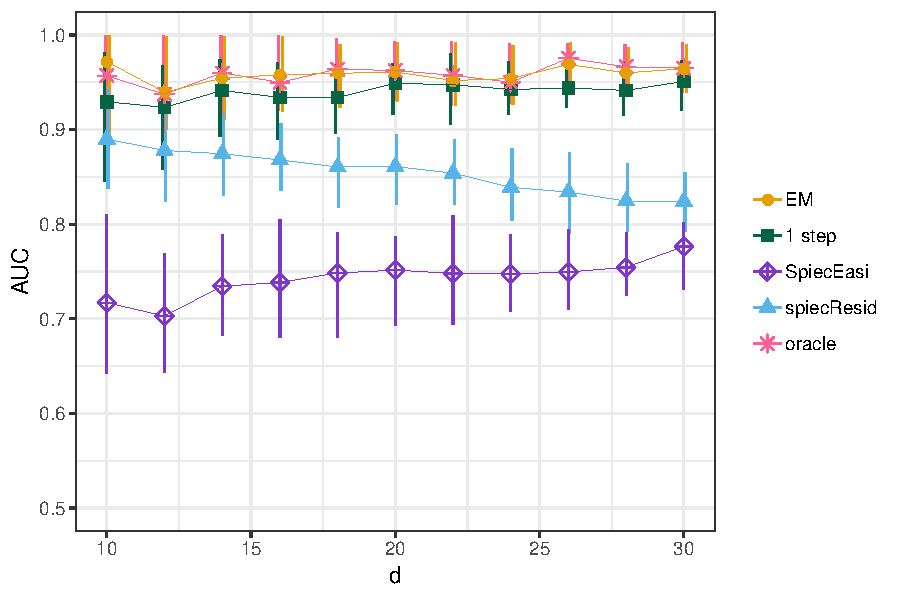
\includegraphics[width=0.25\textwidth]{erdos_d.png}\hspace{1cm}
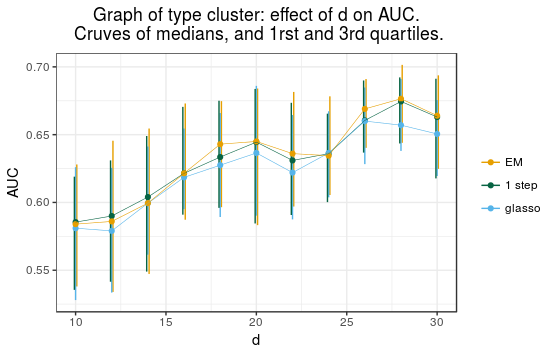
\includegraphics[width=0.25\textwidth]{cluster_d.png}\hspace{1cm}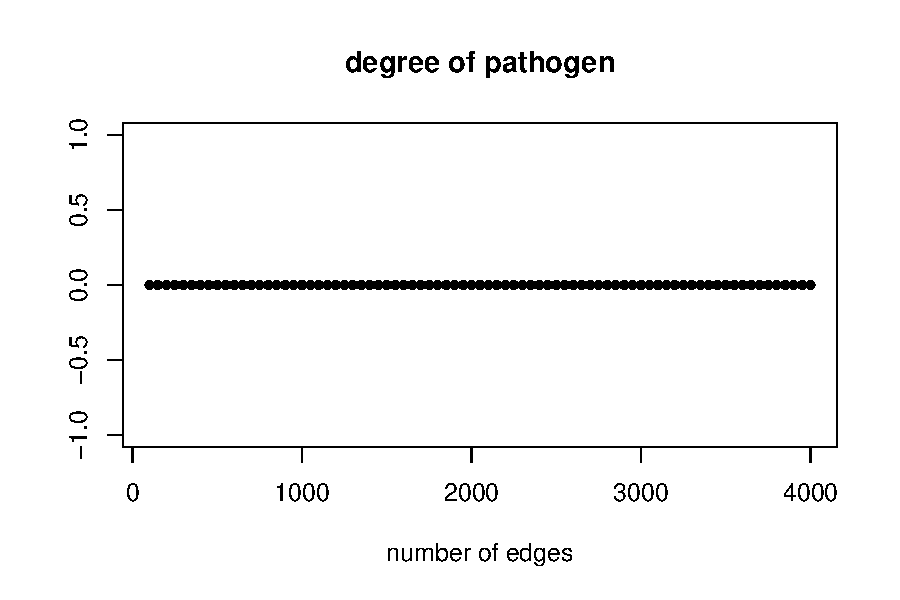
\includegraphics[width=0.25\textwidth]{tree_d.png}\\[2em]

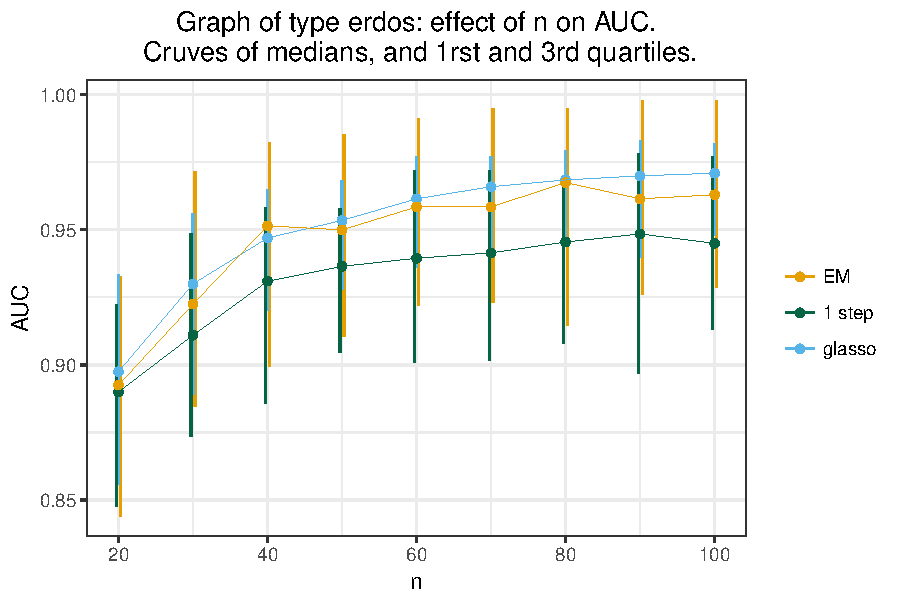
\includegraphics[width=0.25\textwidth]{erdos_n.png}\hspace{1cm}
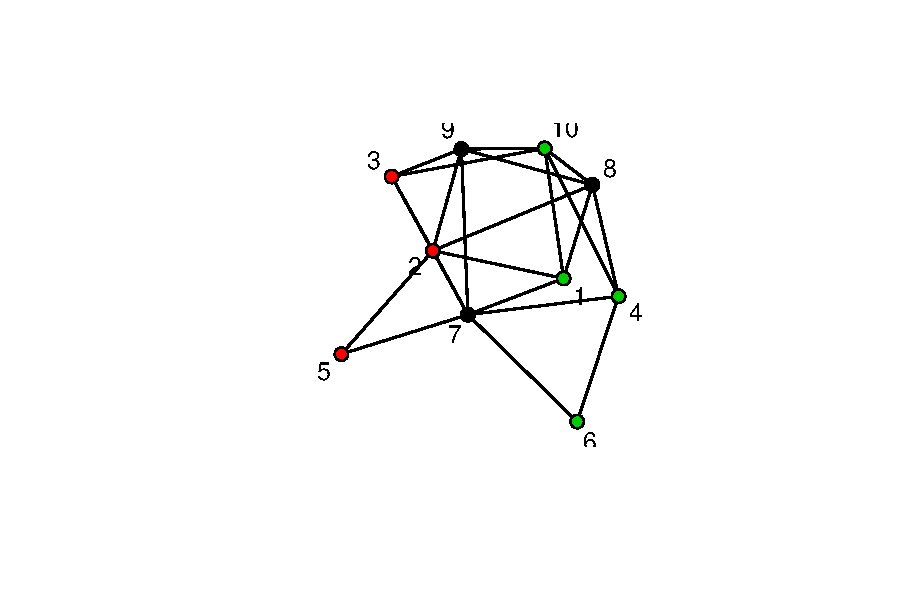
\includegraphics[width=0.25\textwidth]{cluster_n.png}\hspace{1cm}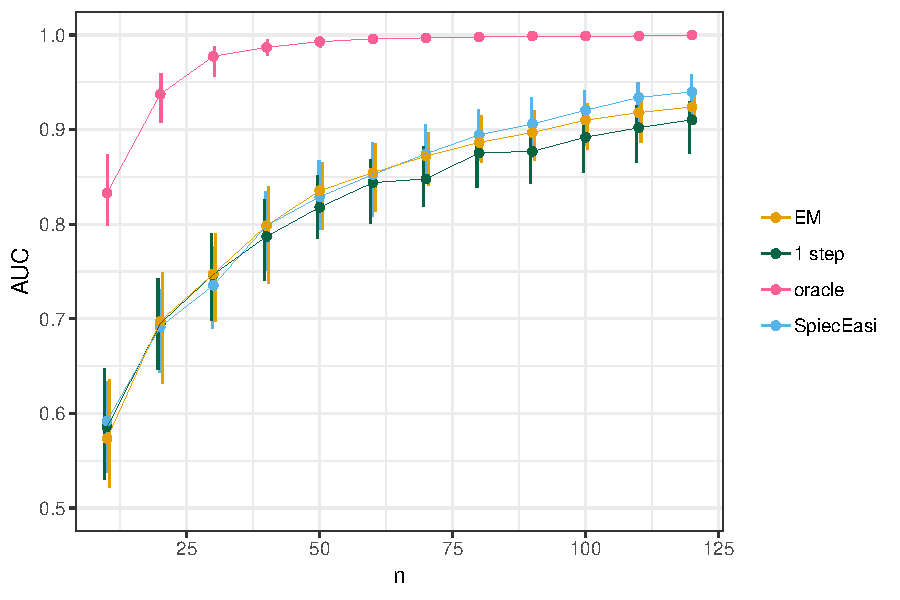
\includegraphics[width=0.25\textwidth]{tree_n.png}\\[2em]
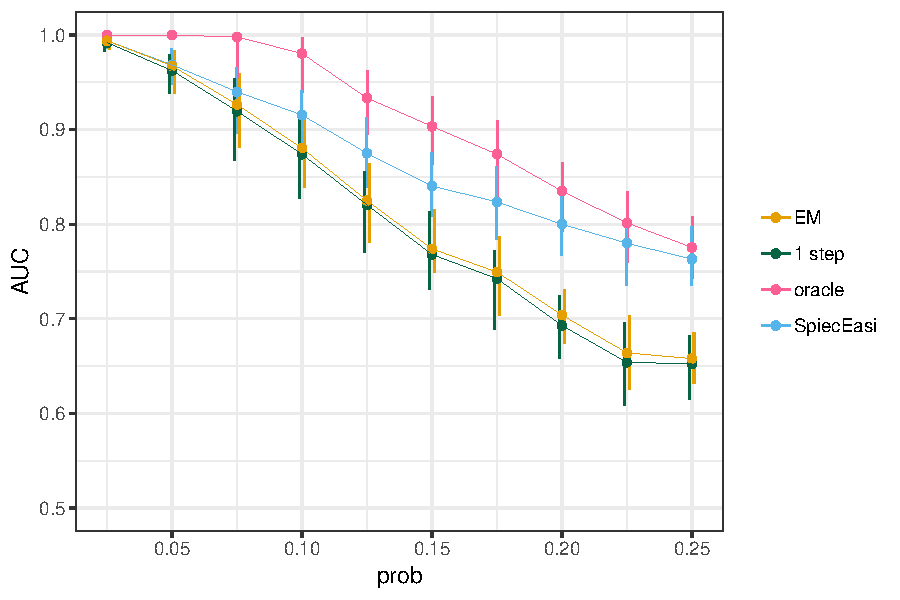
\includegraphics[width=0.25\textwidth]{erdos_prob.png}\hspace{1cm}
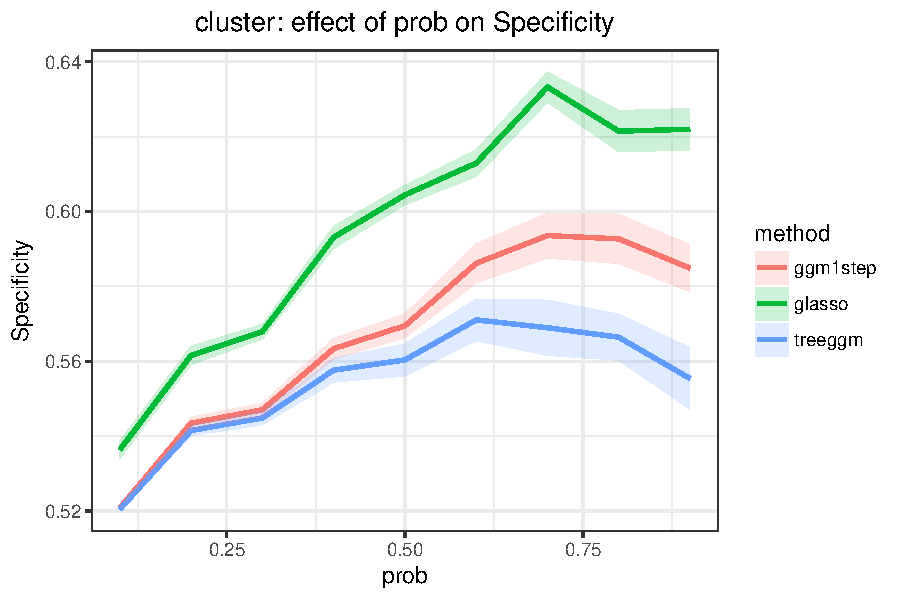
\includegraphics[width=0.25\textwidth]{cluster_prob.png}
\hspace{1cm}    \includegraphics[height = 2cm]{legende.png}\par

\end{frame}

% \begin{frame}{Idée d'estimateur pour $\lambda$}
%    \[Y_i  \sim Y_{\backslash -i}\]
%  
%   \begin{columns}
%    \begin{column}{0.65\linewidth}
%     \begin{itemize}
%         \item Ajuster chaque variable sur l'ensemble des autres %variables
%         \item Nouvelle interprétation des tests des coefficients %en absence vs. présence d'arête : $(\mathcal{H}_0) : %c_{ij} = 0$ vs  $(\mathcal{H}_1) : c_{ij} \neq 0$
%         \item Déduire des p-valeurs un estimateur du nombre de %"non-arêtes"
%     \end{itemize}
%     \end{column}
%     \begin{column}{0.35\linewidth}
%      \pause{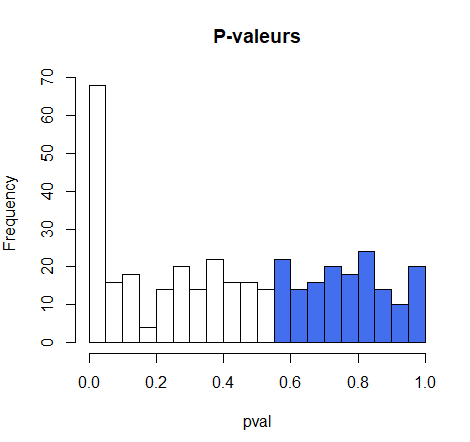
\includegraphics[width=4cm]{histpval.PNG}}
%     \end{column}
%    \end{columns}
%    \pause{
%\begin{block}{$S$ et $S*$}
% \begin{itemize}
%     \item $S*(G)$ : nombre d'absences d'arêtes du graphe $G$
%     \item Estimateur de $S*$ : \[S(Y_G) = 2\sum \mathds{1}\{pval %(Y_G) \geq 1 \} \]
% \end{itemize}
%\end{block}}
%\end{frame}
%
%\begin{frame}{Simulations de $S$}
%   \center{ \includegraphics[width=10cm]{estimate_star.PNG}}
%   \begin{itemize}
%       \item Premiers résultats encourageants
%       \item Semble se dégrader lorsque la probabilité d'arête %augmente dans l'erdos
%   \end{itemize}
%\end{frame}
%\begin{frame}{Estimateur de $\lambda_{seuil}$}
%\begin{itemize}
%    \item  Seuil pour le glasso : \[\hat{\lambda}_{seuil} = %\min_\lambda\{ |S-S_{\lambda}|\},\] avec $S_{\lambda}$ le %nombre d'arêtes annulées pour le seuil $\lambda$. 
%    \item \vspace{1cm} Les scores de l'EM sont des probabilités %d'arêtes : le seuil est la densité estimée de $G$, soit :
%    \[\hat{\beta}_{seuil} = 1 - \frac{2 S}{d(d-1)}\]
%\end{itemize}
%\end{frame}
%\begin{frame}{Exemple}
%Arbre à 7 noeuds : \\
%\begin{center}
%    \includegraphics[width=3cm]{Gtree.PNG}\\
%\end{center}
%
%Résultats :
%    \begin{itemize}
%        \item $S* = 15$, $S=14$
%        \item $\hat{\beta}_{seuil} =0.33$, $\hat{\lambda}_{seuil} %=0.68$
%       \begin{center}
%          \only<1>{  \includegraphics[width=8cm]{bothhist.PNG}}
%          \only<2>{  \includegraphics[width=8cm]{bothgraphs.PNG}}
%       \end{center}
%    \end{itemize}
%\end{frame}
%\begin{frame}{Bilan}
%    \`{A} partir d'un jeu de données :\\ 
%    \vspace{1cm}
%    \begin{itemize}
%        \item un a priori sur la densité du graphe,
%        \item des seuils pour les matrices de scores.
%    \end{itemize}
%    \vspace{1cm}
%La suite :
%    \vspace{1cm}
%    \begin{itemize}
%        \item Comment mesurer l'éloignement à la structure %d'arbre ?
%    \end{itemize}
%\end{frame}
% \section{Suite du sujet}
%%%%%%%%%%%%%%%%%%%%%%%%%%%%%
%%%%%%%%%%%%%%%%%%%%%%%%%%%%%
%%%%%%%%%%%%%%%%%%%%%%%%%%%%%

%\begin{frame}{\'{E}tat de l'art}
%\begin{center}
%    \begin{tikzpicture}
%    [scale=1,->,>=stealth',shorten >=1pt,auto,node %distance=1cm,
%        thick]
%
%     \tikzstyle{every %state}=[draw=none,text=white,scale=1,
%      transform shape] 
%   
%    \node[rect] (A1) at (-2,11) {\Large{GGM }};
%    \node[rect] (A2) at (-2,5)   {\Large{Poisson %log-Normale  }};
%    \node[rect] (A3) at (-2,0)  {\Large{EM}};
%    \node[rect] (A4) at (9,11)  %{\large{Optimisation/Pénalisation}};
%    \node[rect] (A5) at (8,0)  {\Huge{?}};
%    \node[rect] (B1) at (-2,8.5)  {\small{\emph{Données %discrètes}}};
%    \node[rect] (B2) at (1.75,11)  {\small{\emph{Acteur %manquant}}};
%    \node[rect] (B3) at (-2,2.5)  {\small{\emph{Inférence %variationnelle}}};
%    \node[notice={(1,-0.2)}][text width=4cm] at (-3.5,13) %{\small{\cite{Lau96}, \cite{FHT08}, \cite{MeB06}}};
%    \node[notice={(0.6,-0.2)}][text width=2.8cm] at %(-5.5,6.3) {\small{\cite{AiH89}}};
%    \node[notice={(0.7,-0.2)}][text width=2.5cm] at %(-5.5,1) {\small{\cite{CMR17}  }};
%    \node[notice={(-0.2,0.7)}][text width=3.5cm] at %(10,8.2) { \small{\cite{LatentCWP}, \cite{genvieve}}};
%         
%        \draw[connect] 
%        (-1.1,0) -- (7.5,0) ;
%        \draw[connect] 
%        (8,11) -- (8,0.8) ;
%        \draw[-] (A1)  -- (B1);
%        \draw[-] (A1)  -- (B2);
%        \draw[-] (A2)  -- (B3);
%        \draw[->] (B1)  -- (A2);
%        \draw[->] (B3)  -- (A3);
%        \draw[->] (B2)  -- (A4);
%\end{tikzpicture}
%\end{center}
%\end{frame}

%\begin{frame}{Absence d'un acteur principal}
%\only<1>{
%Si un acteur prédominant du réseau n'est pas observé, le %graphe comporte de nouvelles arêtes qui faussent %l'interprétation \cite{LatentCWP} :
%\vspace{0.2cm}
%\begin{columns}
%\begin{column}{0.35\linewidth}
%\begin{center}
%\begin{tikzpicture}
%     
%
%      %% UN graphe 
%      \tikzstyle{every edge}=[-,>=stealth',shorten %>=1pt,auto,thin,draw]
%      \tikzstyle{every node}=[fill=yellow!40!orange]
%      \tikzstyle{every          %state}=[draw=none,text=white,scale=1,
%      transform shape,circular drop shadow] 
%      
%      \node[fill=white] at (2.25,-1) ;
%
%      % premier cluster
%      \node[state] (A1) at (1.2,0) {A};
%      \node[state] (A2) at (2.2,0) {B};
%      \node[state] (A3) at (1.7,1) {C};
%      \node[state] (A4) at (1.7,1) {H};
%      
%        \path (A2) edge [] (A4)
%        (A1) edge [] (A4)
%        (A3) edge [] (A4);
%      
%
%\end{tikzpicture}\\
%
%Graphe complet $\mathcal{G}$
%\end{center}
%\end{column}
%\begin{column}{0.25\linewidth}
%\begin{center}
%$$\underrightarrow{marginalisation}$$
%\end{center}
%
%\end{column}
%\begin{column}{0.35\linewidth}
%\begin{center}
%\begin{tikzpicture}
%     
%
%      %% UN graphe 
%      \tikzstyle{every edge}=[-,>=stealth',shorten %>=1pt,auto,thin,draw]
%      \tikzstyle{every node}=[fill=yellow!40!orange]
%      \tikzstyle{every %state}=[draw=none,text=white,scale=1,
%      transform shape,circular drop shadow] 
%    
%      
%      % premier cluster
%      \node[state] (A1) at (1.2,0) {A};
%      \node[state] (A2) at (2.2,0) {B};
%      \node[state] (A3) at (1.7,1) {C};
%      
%        \path (A2) edge [bend left,] (A1)
%        (A1) edge [bend left] (A3)
%        (A3) edge [bend left] (A2);
%      
%
%\end{tikzpicture}\\
%
%
%Graphe marginal $\mathcal{G}_m$
%\end{center}
%\end{column}
%\end{columns}}
%\vspace{0.2cm}
%$$\mathbf{\mathcal{G}}\text{ : %}\Omega=\underbrace{\begin{pmatrix}
%\Omega_{OO} & \Omega_{OH} \\ 
%\Omega_{HO} & \Omega_{HH}
%\end{pmatrix}}_{\text{arêtes de }E}  \quad %\Sigma=\begin{pmatrix}
%\Sigma_{OO} & \Sigma_{OH} \\ 
%\Sigma_{HO} & \Sigma_{HH}
%\end{pmatrix}$$
%\vspace{0.4cm}
%$$\mathbf{\mathcal{G}_m}\text{ : }\Omega_m= %\underbrace{\Omega_{OO} - %\color{red}\Omega_{OH}\Omega_{HH}^{-1}\Omega_{HO}}_{\tex%t{arêtes de }E_m}\color{black} \quad \Sigma_m = %\Sigma_{OO}$$
%\end{frame}

%\begin{frame}{Avec des données de comptage et acteur %manquant}
%
%
%
%\textbf{Données :}$(Y_{ij})_{i \in \{1,...,n\}, j \in %\{1,...,p+q\}}$: \textit{i} échantillons de $p$ variables %observées, on suppose $q$ variables supplémentaires non %observées.\\
%\vspace{0.3cm}
%\textbf{Modèle :}
%
%\begin{exampleblock}{La loi Poisson log-Normale}
%\[
%            \left.
%                \begin{array}{rl}
%                Z_i \textit{ iid } &\sim %\mathcal{N}_{p+q}(\mu,\Sigma)\\
%                    &(Y_{ij})_j \independent |Z_i\\
%                    Y_{ij}|Z_{ij} &\sim %\mathcal{P}(e^{Z_{ij}}) 
%                   
%                \end{array}
%            \right \} Y \sim \mathcal{P}l\mathcal{N}(\mu, %\Sigma)  
%            \]
%            
%       
%\end{exampleblock}
%\textbf{Méthode :}        
%
%\begin{itemize}
%\item Inclure GGM dans le modèle Poisson-log normal
%\item Inférence variationnelle car $p(Z|Y)$ n'est pas %calculable
%\item Prendre en compte un acteur manquant
%\end{itemize}
%\vspace{0.3cm}
%\textbf{Autres développements envisagés :}
%\begin{itemize}
%    
%\item Prise en compte de covariables
%\item Adapter le modèle à des données recueillies au cours %du temps
%
%\end{itemize}
%\end{frame}
%
\section{Bilan et perspectives}
\begin{frame}{Le modèle A2}
    \begin{itemize}
        \item Modèle A1 : Inférence du réseau latent en deux étapes ( $\hat{\Sigma}_Z$ par {\fontfamily{qcr}\selectfont
PLNmodels} puis inférence du réseau à partir de  $\hat{\Sigma}_Z$)
        \begin{itemize}
        \item Résultats corrects : meilleur ou équivalent au glasso sur un panel de graphes de type et densité différents
            \item facile
            \item Mais l'estimation avec 
{\fontfamily{qcr}\selectfont
PLNmodels} ajoute de la variabilité \vspace{1cm}
        \end{itemize}
        \item Modèle A2 : réécrire le Variational EM utilisé dans {\fontfamily{qcr}\selectfont
PLNmodels}, en y incluant la structure de dépendance par arbre de la couche latente.
         \begin{itemize}
             \item Permettrait de ré-estimer  $\hat{\Sigma}_Z$ à chaque itération
         \end{itemize}
    \end{itemize}
\end{frame}
\begin{frame}{Retour sur la loi PLN}
    
\begin{exampleblock}{La loi Poisson log-Normale}
\[
            \left.
                \begin{array}{rl}
                Z_i \textit{ iid } &\sim \mathcal{N}_{d}(\mu,\Sigma)\\
                    &(Y_{ij})_j \independent |Z_i\\
                    Y_{ij}|Z_{ij} &\sim \mathcal{P}(e^{Z_{ij}}) 
                   
                \end{array}
            \right \} Y \sim \mathcal{PLN}(\mu, \Sigma)  
            \]
            
       
\end{exampleblock}
\vspace{0.5cm}
\begin{itemize}
    \item Le package {\fontfamily{qcr}\selectfont
poilog} de R calcule les densités uni et bi-variées \vspace{0.3cm}
    \begin{itemize}
        \item \large{$\psi_{kl}(Y) = \frac{\mathds{P}(Y_k,Y_l)}{\mathds{P}(Y_k)\times \mathds{P}(Y_l)} $} \normalsize sont directement accessibles
    \end{itemize}

\end{itemize}
\begin{center}
    $\Rightarrow$ Inférence directe du réseau des espèces dans l'espace de Y ?\\
\end{center}

\textbf{Modèle B :}
\[\mathds{P}(Y|T) = \prod_k \mathds{P}(Y_k) \prod_{kl \in T} \mathds{P}(Y_k,Y_l)\]
\end{frame}
\begin{frame}{Perspective}
    \begin{itemize}
    \large{
        \item Choix du seuil des matrices de scores \vspace{0.2cm}
        \item Mise en oeuvre du modèle A2 \vspace{0.2cm}
        \item Confrontation des modèles A et B : Modèles différents avec des marginales identiques ? \vspace{0.2cm}
        \item Prise en compte d'un acteur manquant}
        
    \end{itemize}
    \normalsize
    \pause{
\begin{columns}
\begin{column}{0.35\linewidth}
\begin{center}
\begin{tikzpicture}
     

      %% UN graphe 
      \tikzstyle{every edge}=[-,>=stealth',shorten >=1pt,auto,thin,draw]
      \tikzstyle{every node}=[fill=yellow!40!orange]
      \tikzstyle{every          state}=[draw=none,text=white,scale=0.5,
      transform shape,circular drop shadow] 
      
      \node[fill=white] at (2.25,-1) ;

      % premier cluster
      \node[state] (A1) at (1.2,0) {A};
      \node[state] (A2) at (2.2,0) {B};
      \node[state] (A3) at (1.7,1) {C};
      \node[state] (A4) at (1.7,0.5) {H};
      
        \path (A2) edge [] (A4)
        (A1) edge [] (A4)
        (A3) edge [] (A4);
      

\end{tikzpicture}\\

Graphe complet $\mathcal{G}$
\end{center}
\end{column}
\begin{column}{0.25\linewidth}
\begin{center}
$$\underrightarrow{marginalisation}$$
\end{center}

\end{column}
\begin{column}{0.35\linewidth}
\begin{center}
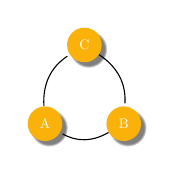
\begin{tikzpicture}
     

      %% UN graphe 
      \tikzstyle{every edge}=[-,>=stealth',shorten >=1pt,auto,thin,draw]
      \tikzstyle{every node}=[fill=yellow!40!orange]
      \tikzstyle{every state}=[draw=none,text=white,scale=0.5,
      transform shape,circular drop shadow] 
    
      
      % premier cluster
      \node[state] (A1) at (1.2,0) {A};
      \node[state] (A2) at (2.2,0) {B};
      \node[state] (A3) at (1.7,1) {C};
      
        \path (A2) edge [bend left,] (A1)
        (A1) edge [bend left] (A3)
        (A3) edge [bend left] (A2);
      

\end{tikzpicture}\\

Graphe marginal $\mathcal{G}_m$
\end{center}
\end{column}
\end{columns}
}
\end{frame}
\begin{frame}{}
\center{\huge{Merci pour votre attention !}\\ \vspace{1cm}
\includegraphics[width=2.2cm]{smile.png}}
    
\end{frame}
%\begin{frame}{Applications}
%
%    \begin{itemize}
%    
%    \item  Comprendre les interactions (compétition, %...) entre les organismes
%    \item Contrôle d'une espèce (d'un pathogène par %exemple)
%\end{itemize}
%\vspace{1cm}
%\begin{alertblock}{Collaborations}
%\begin{itemize}
%    \item Des projets d'écologie microbienne
%    \begin{itemize}
%    \item INRA de Bordeaux avec C. Vacher (pathogène de %la vigne et du chêne)
%    \item INRA de Rennes avec C. Mougel (rhizosphère)
%    \end{itemize}
%    \item Projet ANR Hydrogen (analyse des données du %projet TARA Océan)
%\end{itemize}
%\end{alertblock}
%\vspace{1cm}
%
%\end{frame}



\appendix
\backupbegin
\begin{frame}[allowframebreaks]
 \bibliographystyle{apalike}
    \bibliography{biblio2.bib}
% \frametitle{References}
%\bibliography{cellcite}
\end{frame}

\backupend

\end{document}

